%% --------------------------------------------------------------------------
% LaTeX template for the XLII CILAMCE-PANACME.
%
% This latex document tries to copy the Microsoft Word template.
% --------------------------------------------------------------------------
\documentclass[a4paper,10pt]{book}

% PACKAGES USED - packages that need to be previously installed on your computer
\usepackage[lmargin=2.5cm, rmargin=2.5cm, tmargin=2.5cm, bmargin=2.5cm ]{geometry}
\usepackage{graphicx}
\usepackage{times}
\usepackage{indentfirst}
\usepackage{fancyhdr}
\usepackage{titlesec}
\usepackage[portuguese]{babel}
\usepackage{parskip} 
\usepackage{setspace}
\usepackage{booktabs}
\usepackage{multirow}
\usepackage{float}


%%%%%%%%%%%%%%%%%%%%%%%%%%%%%%%%%%%%%%%%%%%%%%%%%%%%%%%%%%%%%%%%%
%%%%%%%%%%%%%%%%%%%%%%%%%%%%%%%%%%%%%%%%%%%%%%%%%%%%%%%%%%%%%%%%%
%%% My Additional Packages
%%%%%%%%%%%%%%%%%%%%%%%%%%%%%%%%%%%%%%%%%%%%%%%%%%%%%%%%%%%%%%%%%
\usepackage[utf8]{inputenc}
%\usepackage{amssymb} %Mathematics
%\usepackage{amsfonts}%Mathematics
\usepackage{amsmath,amscd}%Mathematics
%\usepackage{amsthm}%Mathematics
%\usepackage{mathrsfs}%Mathematics font
%\usepackage{xspace}
%\usepackage{booktabs}
%\usepackage{stmaryrd}%Particular Brackets
%\usepackage{graphicx} %Tables and Figures
\usepackage{subfigure}
%\usepackage{url}
\usepackage{multirow}
\usepackage{hyperref}
\usepackage{cleveref}
\usepackage{./pkg-crefNames}
\usepackage[labelsep=period]{caption}

%BibTeX compatible with the CILAMCE-PANACM format
\usepackage[numbers,sort&compress]{natbib}

\setlength{\bibsep}{0pt plus 0.3ex}

\renewcommand*{\bibfont}{\small}

\makeatletter
\renewcommand\bibsection
{
  \section*{References}
}



\renewenvironment{thebibliography}[1]
      {\section*{\refname}%
       \@mkboth{\MakeUppercase\refname}{\MakeUppercase\refname}%
       \list{\@biblabel{\@arabic\c@enumiv}}%
            {\settowidth\labelwidth{\@biblabel{#1}}%
             \leftmargin\labelwidth
             \advance\leftmargin-10pt% change 20 pt according to your needs
             \advance\leftmargin\labelsep
             \setlength\itemindent{10pt}% change using the inverse of the length used before
             \@openbib@code
             \usecounter{enumiv}%
             \let\p@enumiv\@empty
             \renewcommand\theenumiv{\@arabic\c@enumiv}}%
       \sloppy
       \clubpenalty4000
       \@clubpenalty \clubpenalty
       \widowpenalty4000%
       \sfcode`\.\@m}
      {\def\@noitemerr
        {\@latex@warning{Empty `thebibliography' environment}}%
       \endlist}
\renewcommand\newblock{\hskip .11em\@plus.33em\@minus.07em}
\makeatother




\makeatother
\bibliographystyle{./bib-cilamce}
%\bibliographystyle{plain}


%%%%%%%%%%%%%%%%%%%%%%%%%%%%%%%%%%%%%%%%%%%%%%%%%%%%%%%%%%%%%%%%%
%%%%%%%%%%%%%%%%%%%%%%%%%%%%%%%%%%%%%%%%%%%%%%%%%%%%%%%%%%%%%%%%%

% CONFIGURATION
\renewcommand*\arraystretch{1.5}
\renewcommand*\thesection{\arabic{section}}
%\hyphenpenalty=10000 % You can uncomment this to avoid hyphenization
\titleformat*{\section}{\large\bfseries}
\titleformat*{\subsection}{\bfseries}
\titlespacing\section{0pt}{20pt plus 2pt minus 2pt}{12pt plus 2pt minus 2pt}
\titlespacing\subsection{0pt}{20pt plus 0pt minus 0pt}{12pt plus 0pt minus 0pt}
\setlength{\parskip}{0pt} % Spacing between paragraphs
\setlength{\parindent}{0.75cm} % Paragraph identation
\setlength\abovecaptionskip{6pt}

% --------------------------------------------------------------------------
% DO NOT EDIT - SPECIAL HEADINGS OF XLI CILAMCE-PANACM
% --------------------------------------------------------------------------
\fancypagestyle{first}
{
\fancyhf{}
\fancyfoot[RO]{\footnotesize \textit{Universidade Federal de Alagoas - UFAL \\
Programa de Pós-graduação em Enegenharia Civil - PPGEC/UFAL \\
Introdução à Engenharia do Petróleo - EES149 \\
Maceió, Alagoas, 04 de Março de 2022}}
\renewcommand{\headrulewidth}{.0pt}
\renewcommand{\footrulewidth}{.5pt}
}


\pagestyle{fancy}
\fancyhf{}

\fancyfoot[LE]{\footnotesize \textit{Universidade Federal de Alagoas - UFAL \\
Programa de Pós-graduação em Enegenharia Civil - PPGEC/UFAL \\
Introdução à Engenharia do Petróleo - EES149 \\
Maceió, Alagoas, 04 de Março de 2022}}

\fancyfoot[RO]{\footnotesize \textit{Universidade Federal de Alagoas - UFAL \\
Programa de Pós-graduação em Enegenharia Civil - PPGEC/UFAL \\
Introdução à Engenharia do Petróleo - EES149 \\
Maceió, Alagoas, 04 de Março de 2022}}




\renewcommand{\headrulewidth}{.5pt}
\renewcommand{\footrulewidth}{.5pt}

% --------------------------------------------------------------------------
% PLEASE, EDIT THIS!
%\fancyhead[LE]{\footnotesize \textit{Avaliação da integridade de elemento de barreira de poço em cenários de $kick$ de gás e perda de circulação total}}
\fancyhead[LE]{\footnotesize \textit{Integridade de elemento de barreira de poço em cenários de perfuração: um estudo de caso}}
\fancyhead[RO]{\footnotesize \textit{G. L. L. Santos, O. B. A. Rodrigues, J. P. L. Santos}}
% --------------------------------------------------------------------------

\begin{document}\thispagestyle{first}

% --------------------------------------------------------------------------
% DO NOT EDIT - LOGO OF XLI CILAMCE
% --------------------------------------------------------------------------

\begin{figure}[ht!]
\vspace{-30pt}
%\flushright
\center

\includegraphics[width=15.0cm]{Figures/cab}
\vspace{10pt}
\end{figure}

% --------------------------------------------------------------------------
% TITLE OF PAPER
% --------------------------------------------------------------------------

\noindent
%\textbf{\Large
%Avaliação da integridade de elemento de barreira de poço em cenários de \textit{kick} de gás e perda de circulação total} 
\textbf{\Large
Integridade de elemento de barreira de poço em cenários de perfuração: um estudo de caso} 
\vspace{18pt} % <- keep this vertical space!

% --------------------------------------------------------------------------
% AUTHORS
% --------------------------------------------------------------------------

\noindent Gilberto L. L. Santos$^1$, Otávio B. A. Rodrigues$^1$, João P. L. Santos$^1$

\vspace{18pt} % <- keep this vertical space!


\noindent $^1$\textit{Laboratório de Computação Científica e Visualização, Centro de Tecnologia, Universidade Federal de Alagoas, LCCV/CTEC/UFAL}

\noindent \textit{Campus A. C. Simoes, 57072-970, Maceió/Alagoas, Brazil}

\noindent \textit{gilberto.santos@lccv.ufal.br, otavio.rodrigues@lccv.ufal.br, jpls@lccv.ufal.br}


\vspace{18pt} % <- keep this vertical space!

% --------------------------------------------------------------------------
% ABSTRACT
% --------------------------------------------------------------------------

\noindent \textbf{Resumo.}
This template file provides detailed formatting instructions for preparing your full-length paper to the Proceedings of the joint CILAMCE-PANACM-2021 (XLII Ibero-Latin American Congress on Computational Methods in Engineering and III Pan-American Congress on Computational Mechanics). It is strongly recommended that you use the pre-defined styles of this template file, as they embed all necessary text formatting for the corresponding paragraph type. Full-length papers must be written in English.

\vspace{18pt} % <- keep this vertical space!

\noindent \textbf{Palavras-chave:} First keyword, Second keyword, Third keyword (up to 5 keywords)


% --------------------------------------------------------------------------
\section{Introdução}\label{sec:introduction}
% --------------------------------------------------------------------------
%O objetivo deste trabalho é avaliar a integridade de poços com base na avaliação de sistemas de barreiras de segurança, durante as atividades de perfuração do poço. Com relação ao procedimento de perfuração, em poços de petróleo utilizam-se sondas de perfuração, que consistem em um conjunto de equipamentos, que podem variar quanto a sua tipologia \cite{cardoso}. A Figura \ref{fig: perf_esquema} ilustra um esquema geral da sonda na perfuração de poços. 

%\begin{figure}[!ht]
%\begin{center}
%\includegraphics[scale=0.5]{Figures/%perf_esquema2.pdf}
%\vspace{12pt}
%\caption{Esquema geral da sonda na perfuração. %Fonte:  \citep{perf_esquema}.}
%\label{fig: perf_esquema}
%\end{center}
%\end{figure}
%\vspace{8pt}

%O poço é perfurado em várias fases, que são revestidas e formam as colunas de revestimento, iniciando com um tubo de pequena extensão e diâmetro maior que os posteriores. Para realizar a perfuração da fase, é necessário um conjunto de ferramentas que constitui a coluna de perfuração, tais como os tubos de perfuração e as brocas, além disso, utiliza-se o fluido de perfuração, também chamado de lama de perfuração. Estabilizar a parede da formação rochosa e carrear os cascalhos cortados pela broca são alguns dos objetivos do fluido de perfuração \cite{paranhos}.


%Para obter uma perfuração estável e segura, reduzindo problemas operacionais, é necessário manter o peso do fluido de perfuração maior que a pressão de poros e de colapso e menor que a pressão de fratura. Nesse contexto, se essa pressão no poço se tornar menor que a pressão na formação e, se esta possuir permeabilidade suficiente, acontecerá um $kick$, ou seja, um fluxo indesejado de fluido da formação para o interior do poço \cite{Iago}. 

%De acordo com \cite{lindi2017analysis}, existem métodos de detecção de $kick$, tais como: um aumento na taxa de fluxo de retorno de lama; aumento da taxa de penetração e fluxo do poço com as bombas desligadas. Uma vez detectado o $kick$, métodos de controle são utilizados para reestabelecer o contróleo primário do poço, restaurando o equilíbrio hidrostático, pode-se citar os métodos convencionais (Método do Sondador, Método do Engenheiro e Métodos Volumétricos) e não convencionais (Bullheading, Stripping e Snubbing) \cite{Iago}.

Um poço de petróleo é perfurado em várias fases, que são revestidas e formam as colunas de revestimento, iniciando com um tubo de pequena extensão e diâmetro maior que os posteriores. Para realizar a perfuração da fase, é necessário um conjunto de ferramentas que constitui a coluna de perfuração, além do fluido de perfuração. De acordo com \citep{thomas2001fundamentos}, quando a pressão do fluido é inferior a pressão de poros dos fluidos confinados nos poros há um influxo destes para o poço, formando um $kick$. \citep{thomas2001fundamentos} ainda explica que um fluxo indesejado da formação de forma incontrolável gera um $blowout$, conforme ilustrado nas setas da Figura~\ref{fig:graph}.

Adicionalmente, a Figura~\ref{fig:graph} mostra a ocorrência de $blowout$ no ciclo de vida de poços no Golfo do México, Reino Unido (UK) e no Mar do Norte. Segundo \citep{SINTEF}, geralmente, os dados das plataformas dessas regiões são mais bem documentados do que explosões em outras localidades. É percebida que, para o período analisado, mais da metade dos $blowouts$ aconteceram durante a etapa de perfuração. Dessa forma, tem-se a importância de dedicar estudos para mitigar o problema em questão.

\begin{figure}[H]
\begin{center}
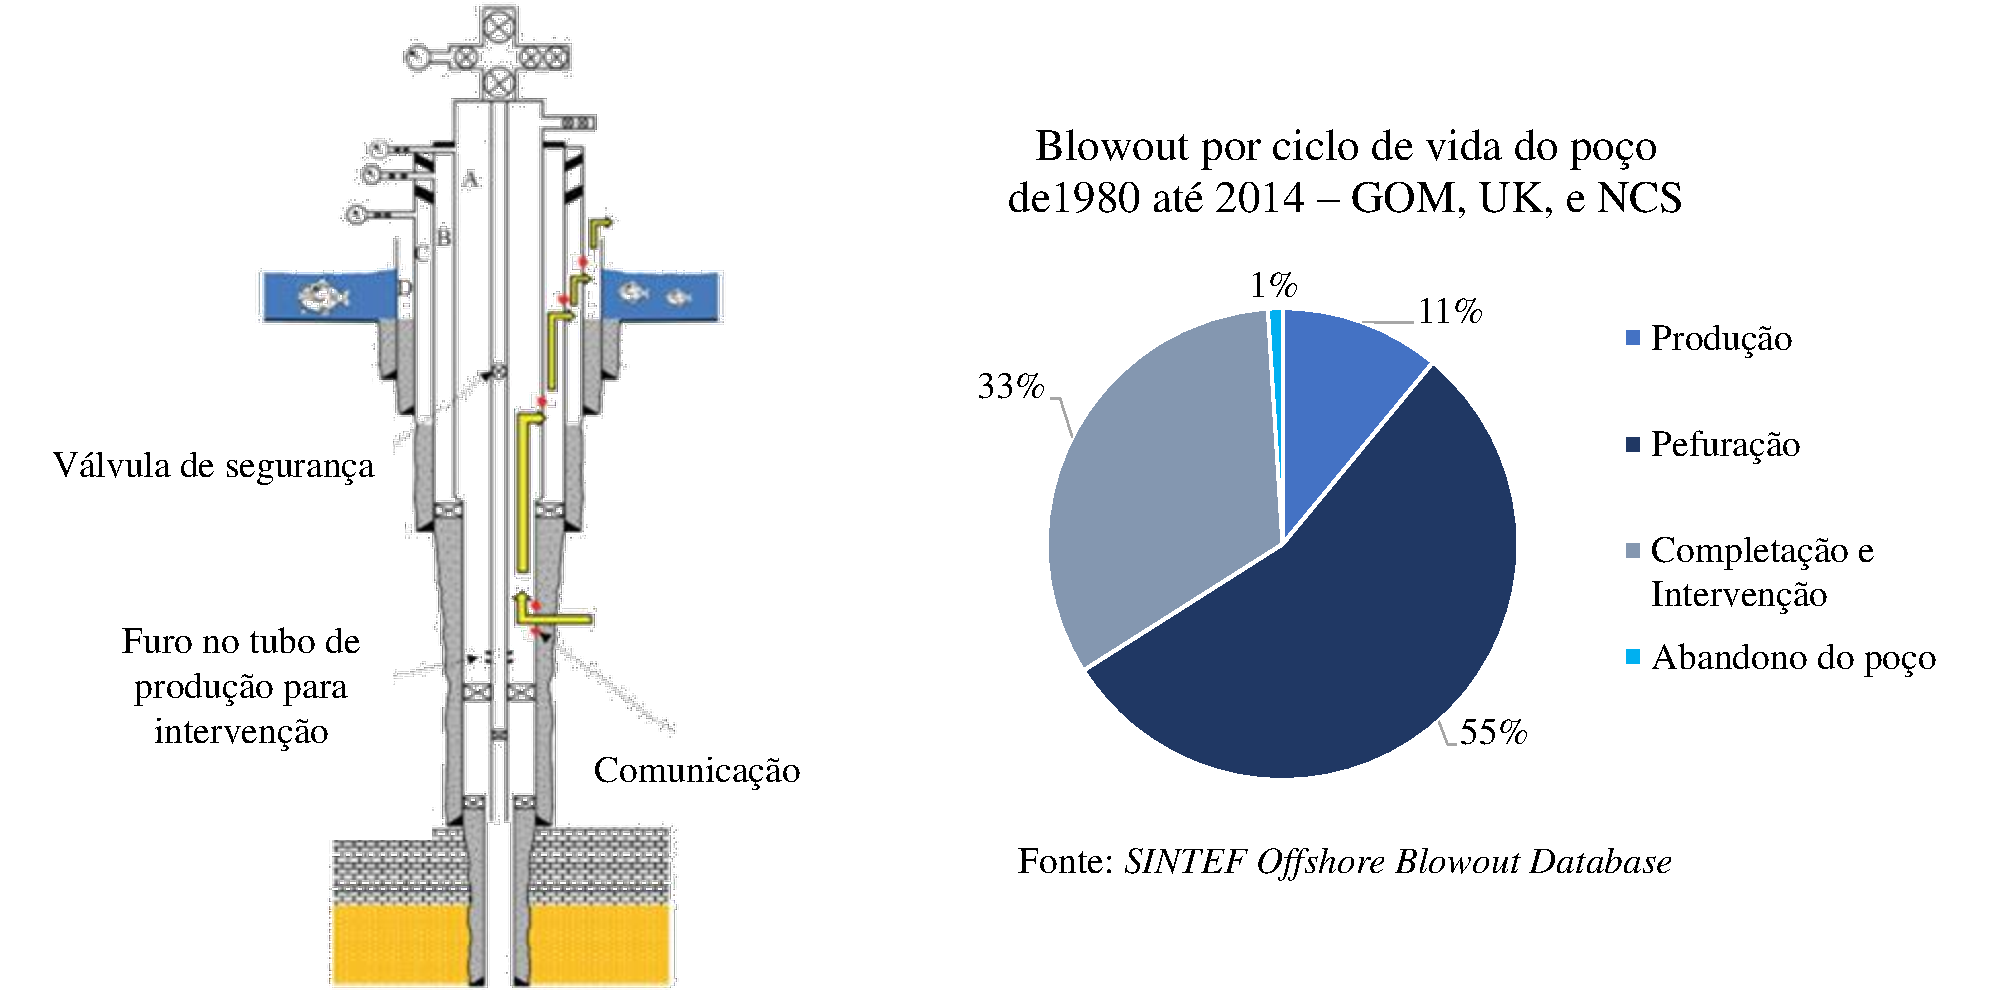
\includegraphics[scale=0.35]{Figures/poco2_teste.pdf}
\vspace{12pt}
\caption{\centering{Esquema da evolução de um $kick$ para um $blowout$. Fonte: Adaptado de \citep{inbook}. $Blowout$ no ciclo de vida de poços.}}
\label{fig:graph}
\end{center}
\end{figure}
\vspace{8pt}


Segundo \citep{santana2021kick}, um $blowout$ é capaz de causar danos aos equipamentos da sonda, assim como lesões às pessoas que trabalham nela. Em 2010, por exemplo, um $blowout$ ao perfurar o poço de Macondo no golfo do México gerou incêndios e explosões na plataforma que levaram a morte de onze pessoas, além do vazamento de quase 5.000.000 de barris de óleo \citep{nunes2015impactos}. No Brasil, segundo relatório final da ANP \cite{ANP}, um $underground$ $blowout$ (o fluxo de fluidos ocorre de uma formação para outra) em um poço do campo de Frade foi a causa do vazamento de 3.700 barris de petróleo cru no mar.   

Estes e outros incidentes fizeram com que a ANP propusesse a resolução nº 46/2016, na qual são estabelecidos os requisitos e diretrizes para a implementação e operação de um Sistema de Gerenciamento da Integridade de Poços (SGIP) de forma a proteger a vida humana e o meio ambiente, à integridade dos ativos da união, de terceiros e do operador do contrato \citep{resolucao}. No SGIP é importante o funcionamento do Conjunto Solidário de Barreiras (CSB) que se refere a um ou mais elementos de barreira de poço capazes de controlar $kick$ ou $blowout$. O CSB é classificado em primário ou segundário. 

A falha dos elementos do conjunto primário torna necessária uma intervenção através dos elementos do conjunto secundário. A Figura \ref{Fig2} mostra os elementos de barreira de poço dos CSB primário e secundário durante a perfuração. Entre tais, destacam-se o fluido na coluna e o revestimento. É importante garantir a integridade dessas estruturas. A variação permitida para as pressões do fluido de perfuração no poço, segundo \citep{rocha2009projeto}, deve obedecer a janela operacional, ou seja, respeitar os limites das pressões de poros, fratura e colapso. As colunas de revestimento, de acordo com \citep{aadnoy2010modern},  são dimensionadas para suportar $burst$ e colapso, além de esforços à tração.

\begin{figure}[H]
\begin{center}
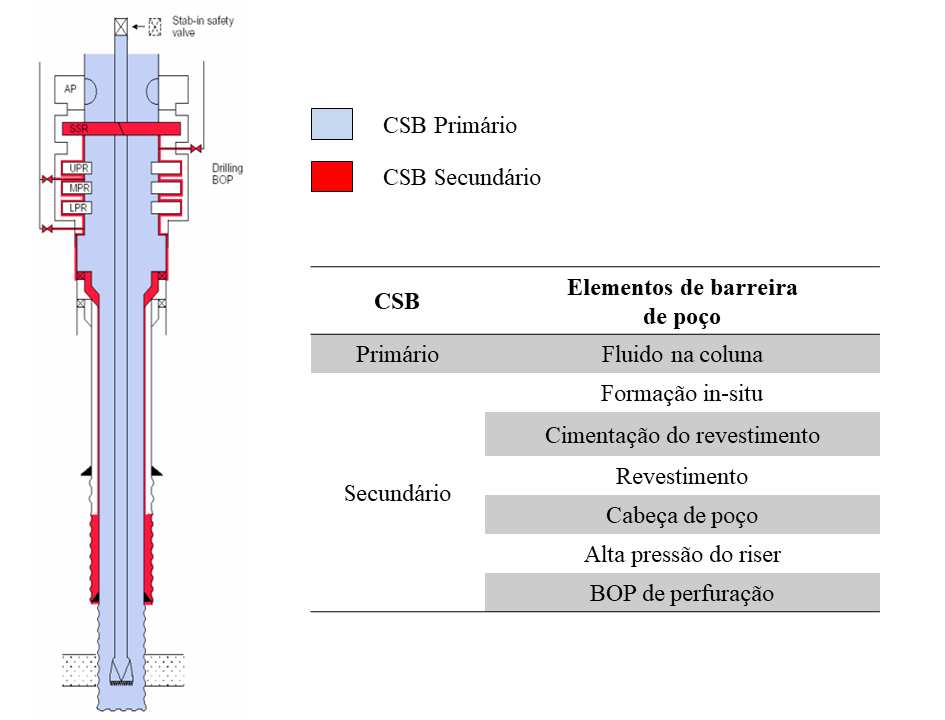
\includegraphics[scale=0.37]{Figures/CSB_corrigido.png}
\vspace{12pt}
\caption{Elementos de barreira de poço em um processo de perfuração. Fonte: Adaptado de \citep{norge2013norsok}.}
\label{Fig2}
\end{center}
\end{figure}
\vspace{8pt}


Na literatura são encontrados alguns trabalhos que envolvem a integridade em fluidos e revestimento. \cite{mendesanalise}, por exemplo, analisam diferentes critérios de assentamento de sapatas de revestimento e definem o peso de fluido de perfuração ótimo a partir da média entre as pressões de poros e de fratura.  \citep{melo2019integrated}, \citep{tenorio} e \citep{tenoriosoeaa}, por exemplo, avaliam a possibilidade de falha em revestimentos considerando os cenários de $kick$ de gás durante a perfuração, cimentação na instalação e uma análise integrada de $kick$ e cimentação, respectivamente. Para tanto, utiliza-se a ferramenta $Casing$ $Well$ (CWELL), a qual foi desenvolvida por \citep{costa} e está disponível no Sistema de Aplicações de Engenharia de Petróleo (SAEP).

%Neste contexto, o objetivo do trabalho é uma análise da integridade de elementos de barreira do CSB primário e secundário durante as fases de perfuração. Para tanto, é realizado o estudo de caso de um poço, analisando diferentes fluidos de perfuração e verificando a formação de $kick$ segundo o critério de janela operacional. Além disso, é avaliada a possibilidade de falha nos revestimentos por meio do $CWELL$, considerando os cenários de $kick$ de gás, poço completo de gás e perda de circulação total. 

Neste contexto, o objetivo do trabalho é uma análise da integridade de elementos de barreira do CSB secundário durante a fase de perfuração. Para tanto, é realizado o estudo de caso de um poço, admitindo a falha no CSB primário e focando no elemento de barreira secundária de revestimentos. Assim, é avaliada a possibilidade de falha nos revestimentos do poço por meio do CWELL, considerando os cenários de $kick$ de gás e perda de circulação total. A principal contribuição deste trabalho em relação aos anteriores é uma análise da integridade do revestimento por meio de um cenário de perda de circulação total, utilizando o CWELL. 

% --------------------------------------------------------------------------
\section{Projeto de revestimento de poços}\label{sec:cen}
% --------------------------------------------------------------------------

Como mencionado anteriormente, as colunas de revestimento são dimensionadas, considerando tração, $burst$ e colapso. Neste sentido, o API TR 5C3 \citep{american2008technical} estabelece a resistência à tração $R_{t}$ como 

%O CWELL estabele a resistência a esses carregamentos conforme a API TR 5C3 \citep{american2008technical}. Neste sentido, a resistência à tração $R_{t}$ é dada por 

%\vspace{6pt}
\begin{center}
\begin{equation}
R_{t} = A_{s}Y_{p},
\label{Eq1}
\end{equation}
\end{center}
%\vspace{6pt}

\noindent onde $A_{s}$ e $Y_{p}$ são a área da seção transversal e a tensão mínima de escoamento do revestimento. Por outro lado, a resistência ao $burst$ $R_{b}$ é obtida por

%\vspace{6pt}
\begin{center}
\begin{equation}
R_{b} = 2Y_{p}\frac{0,875t}{D},
\label{Eq2}
\end{equation}
\end{center}
%\vspace{6pt}

\noindent em que $t$ e $D$ são a espessura e o diâmetro externo do revestimento. É importante destacar que o coeficiente 0,875 da Eq. (\ref{Eq2}) significa uma penalização devido às imperfeições do material durante a fabricação de tubos.

O colapso das colunas de revestimento pode ocorrer nos regimes de escoamento, plástico, transição e elástico.  Sendo assim, para cada um destes há uma resistência ao colapso $R_{cesc}$, $R_{ct}$, $R_{ce}$ e $R_{cp}$, respectivamente, conforme abaixo:

%\vspace{6pt}
\begin{center}
\begin{equation}
R_{cesc} = 2Y_{p} \left [ \dfrac{\left ( \dfrac{D}{t} \right )-1}{\left ( \dfrac{D}{t} \right )^2} \right ],
\label{Eq1}
\end{equation}
\end{center}
%\vspace{6pt}
%\vspace{6pt}

\begin{center}
\begin{equation}
R_{ct} = Y_{p}\left [ \dfrac{A}{\left ( \dfrac{D}{t} \right )} - B \right ] - C,
\label{Eq1}
\end{equation}
\end{center}

%\vspace{6pt}
%\vspace{6pt}
\begin{center}
\begin{equation}
R_{ce} = Y_{p}\left [ \dfrac{F}{\left ( \dfrac{D}{t} \right )} - G \right ],
\label{Eq1}
\end{equation}
\end{center}
%\vspace{6pt}
%\vspace{6pt}

\begin{center}
\begin{equation}
R_{cp} = \dfrac{46,95\cdot 10^6}{ \dfrac{D}{t}\left[ \left ( \dfrac{D}{t} \right )-1 \right ]^2},
\label{Eq1}
\end{equation}
\end{center}
%\vspace{6pt}

\noindent onde $A$, $B$, $C$, $F$ e $G$ são constantes obtidas por equações empíricas em função da tensão de escoamento. É importante destacar que o regime de colapso vigente no revestimento varia conforme a relação entre o diâmetro externo e a espessura do revestimento, além das constantes $A$, $B$, $C$, $F$ e $G$. Em API TR 5C3 \citep{american2008technical} são apresentadas as relações para cada regime, assim como as equações das constantes. 

Também é possível avaliar a resistência de forma tridimensional, a partir do critério de falha de von Mises. Assim, são feitas algumas considerações como definição de tensões em cilindros e características específicas do cenário de $burst$ e colapso, resultando nas seguintes expressões para as pressões por $burst$ ($P_{burst}$) e colapso ($P_{colapso}$):


\begin{center}
\begin{equation}\label{Eq6}
P_{burst} = \dfrac{d^2\sigma_{z}+\sqrt{3D^4Y_p^2-9D^4\tau_{ha}^2-3D^4\sigma_z^2-Y_p^2d^4-3d^4\tau_{ha}^2}(D^2-d^2)}{3D^4+d^4},
\end{equation}
\end{center}

\begin{center}
\begin{equation}\label{Eq8}
P_{colapso} = - \dfrac{\sigma_{z}+\sqrt{4Y_{p}^2-12\tau_{ha}^2-3\sigma_{z}^2}(D^2-d^2)}{4D^2},
\end{equation}
\end{center}


\noindent em que $d$ é o diâmetro interno do revestimento, $\sigma_{eq}$,  $\sigma_{z}$, $\sigma_{h}$, $\sigma_{r}$, $\tau_{ha}$ são as tensões de von Mises, axial, tangencial, radial e cisalhamento torcional, respectivamente. As equações (\ref{Eq6}) e (\ref{Eq8}) correspondem a parte superior e inferior da elipse triaxial de von Mises ilustrada na Figura \ref{poco2}, a qual delimita uma região onde o revestimento possui um comportamento elástico. \citep{costa} mostra em detalhes o passo a passo para atingir as equações anteriores. Além disso, o API TR 5C3 \citep{american2008technical} fornece uma envoltória de segurança, a qual é resultado das resistências acima, dos fatores de segurança e está ilustrada também na Figura \ref{poco2}. Esses dois métodos compõem uma análise triaxial.


\begin{figure}[H]
\begin{center}
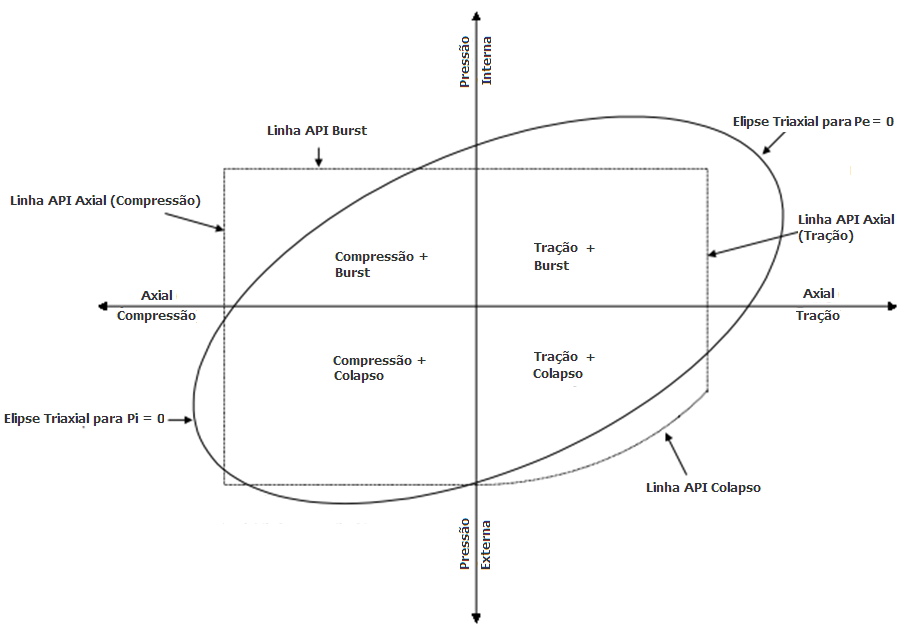
\includegraphics[scale=0.4]{Figures/elipse.png}
%\vspace{12pt}
\caption{Elipse de resistência triaxial de revestimento. Fonte: \cite{costa}.}
\label{poco2}
\end{center}
\end{figure}



%\vspace{6pt}
%\begin{center}
%\begin{equation}
%A = 2,8762 + 0,10679\cdot 10^{-5}\cdot Y_{p} + 0,21301 %\cdot 10^{-10} \cdot {Y_{p}}^2 - 0,53132 \cdot 10^{-16} \cdot {Y_p}^3,
%\label{Eq1}
%\end{equation}
%\end{center}
%\vspace{6pt}
%\vspace{6pt}

%\begin{center}
%\begin{equation}
%B = 0,026233 + 0,50609 \cdot 10^{-6} \cdot Y_{p},
%\label{Eq1}
%\end{equation}
%\end{center}

%\vspace{6pt}
%\vspace{6pt}
%\begin{center}
%\begin{equation}
%C = -465,93 + 0,030867 \cdot Y_{p} - 0,10483 \cdot 10^{-7} \cdot {Y_{p}}^2 + 0,36989 \cdot 10^{-13} \cdot {Y_{p}}^3,
%\label{Eq1}
%\end{equation}
%\end{center}
%\vspace{6pt}
%\vspace{6pt}

%\begin{center}
%\begin{equation}
%F = \dfrac{46,95\cdot 10^6 \left [ \dfrac{\left ( %%\dfrac{3B}{A} \right )}{2+\left ( \dfrac{B}{A} \right )} \right ]^3}{Y_{p}\left [ \dfrac{\left ( \dfrac{3B}{A} \right )}{2+\left ( \dfrac{B}{A} \right )} -\dfrac{B}{A} \right ]\left [ 1- \dfrac{\left ( \dfrac{3B}{A} \right )}{2+\left ( \dfrac{B}{A} \right )} \right ]^2},
%\label{Eq1}
%\end{equation}
%\end{center}
%\vspace{6pt}

%\begin{center}
%\begin{equation}
%G = \dfrac{FB}{A}.
%\label{Eq1}
%\end{equation}
%\end{center}
%\vspace{6pt}

%É importante destacar que o regime de colapso vigente no revestimento é determinado conforme a relação entre o diâmetro externo e a espessura do revestimento, além de equações empíricas envolvendo as constantes $A$, $B$, $C$, $F$ e $G$. Em API TR 5C3 \citep{american2008technical} são apresentadas as relações para cada regime. 

%Também é possível avaliar a resistência de forma tridimensional, a partir do critério de falha de von Mises:

%\begin{center}
%\begin{equation}
%\sigma_{eq}=\dfrac{1}{\sqrt{2}}\sqrt{(\sigma_{z}-%\sigma_{h})^2+(\sigma_{h}-\sigma_{r})^2+6\tau_{ha} },
%\label{Eq1}
%\end{equation}
%\end{center}

%\noindent em que $\sigma_{eq}$,  $\sigma_{z}$, $\sigma_{h}$, $\sigma_{r}$, $\tau_{ha}$ são as tensões de von Mises, axial, tangencial, radial e cisalhamento torcional, respectivamente. Assim, são feitas algumas considerações como a definição de tensões em cilindros e características específicas do cenário de $burst$ e colapso. Em \citep{costa}, por exemplo, é mostrado em detalhes o passo a passo. Além disso, a API TR 5C3 \citep{american2008technical} fornece uma envoltória de segurança, a qual é resultado das resistências acima e de fatores de segurança. Esses dois métodos compõem uma análise triaxial.


%Em \citep{costa} é mostrado em detalhes o passo a passo para atingir as equações anteriores. Além disso, a API TR 5C3 \citep{american2008technical} fornece uma envoltória de segurança, a qual é resultado das resistências acima e de fatores de segurança. Esses dois métodos compõem uma análise triaxial.

O método de análise triaxial permite a avaliação simultânea da integridade do
revestimento com base nos cenários críticos de esforços que o sistema de revestimento deve suportar.
Os esforços atuantes ao longo da profundidade do revestimento são representados graficamente por
pares ordenados (esforço axial, pressão diferencial). Para garantia de atendimento de integridade
estrutural do sistema, os valores plotados dos pares ordenados (esforço axial, pressão diferencial)
devem estar contidos no espaço delimitado pela envoltória da elipse de von Mises e pela envoltória de
segurança API \citep{santos2021desenvolvimento}. Os procedimentos apresentados anteriormente são a base dos cálculos realizados pelo CWELL a fim de avaliar ou dimensionar revestimentos com a possibilidade de adicionar os fatores de segurança.


%  --------------------------------------------------------------------------
\section{Cenários de barreira de segurança} \label{sec:cenários}
% --------------------------------------------------------------------------

O cenário de estudo adotado é apresentado na Figura~\ref{fig:poco}. A Tabela~\ref{tab:poco} apresenta os valores numéricos associados a configuração do poço adotado. Os fatores de segurança estão disponíveis na Tabela~\ref{tab:fatores}. Este caso de estudo é semelhante ao apresentado por \citep{costa}. Neste trabalho é avaliada a perda total de circulação nas fases 1 (revestimento condutor) e 2 (revestimento de superfície). Adicionalmente, na terceira fase (revestimento intermediário), é avaliado um cenário de \textit{kick} de gás.  

A perda de circulação é a invasão de fluido de perfuração para a formação através de fraturas existentes ou provocadas em formações com alta permo-porosidade (devido à presença de formação inconsolidada, existência de falhas, fraturas naturais, cavernas, entre outros) ou em zonas depletadas \citep{Chieza2011}. Na perda de circulação total não há retorno do fluido para a superfície. Neste caso, tem-se uma falha no CSB primário (fluido de perfuração), pois a invasão da lama na formação reduz o nível de fluido de perfuração no anular, diminuindo a pressão hidrostática \citep{Chieza2011}. Caso pressão hidrostática alcançar níveis abaixo da pressão de poros, a perda total de circulação pode ocasionar um \textit{kick}. Admitindo que a barreira primária seja rompida, as resistências dos revestimentos que compõem o poço são analisadas, observe na Figura~\ref{Fig2} que o revestimento é um dos elementos dos CSB secundário.

\begin{figure}[H]
\begin{center}
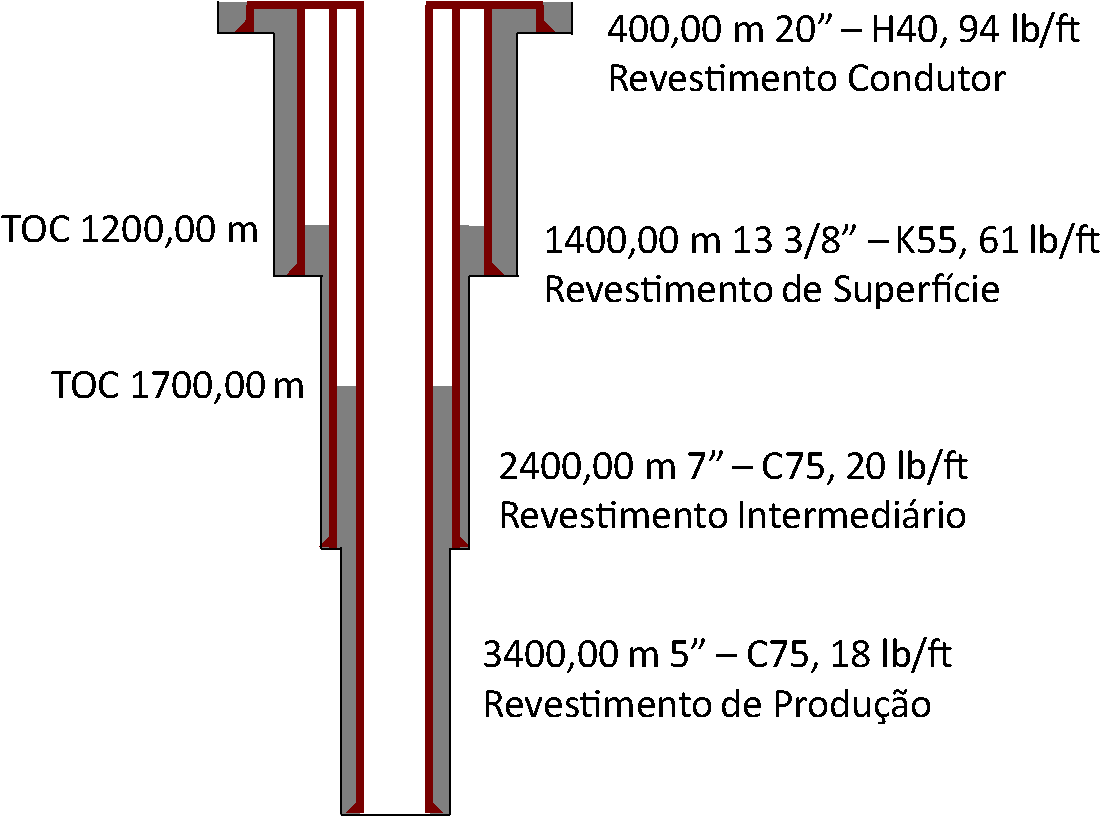
\includegraphics[scale=0.4]{Figures/poco.pdf}
%\vspace{12pt}
\caption{Esquema do modelo do poço.}
\label{fig:poco}
\end{center}
\end{figure}



% Please add the following required packages to your document preamble:
% \usepackage{multirow}
\begin{table}[H]
\centering
\caption{Valores numéricos associados ao caso de estudo. Fonte: Adaptado de \citep{costa}.}
\label{tab:poco}
\begin{tabular}{ccccccccc}
\multicolumn{1}{c|}{\multirow{2}{*}{Revestimento}} & \multicolumn{1}{c|}{\multirow{2}{*}{\begin{tabular}[c]{@{}c@{}}Diâmetro\\  Externo {[}pol{]}\end{tabular}}} & \multicolumn{3}{c|}{MD {[}m{]}} & \multicolumn{1}{c|}{\multirow{2}{*}{\begin{tabular}[c]{@{}c@{}}Broca \\ {[}pol{]}\end{tabular}}} & \multicolumn{1}{c|}{\multirow{2}{*}{\begin{tabular}[c]{@{}c@{}}Densidade \\ da lama {[}lb/gal{]}\end{tabular}}} & \multicolumn{1}{c|}{\multirow{2}{*}{Grade}} & \multirow{2}{*}{\begin{tabular}[c]{@{}c@{}}Peso \\ linear {[}lb/ft{]}\end{tabular}} \\ \cline{3-5}
\multicolumn{1}{c|}{} & \multicolumn{1}{c|}{} & Hanger & TOC & \multicolumn{1}{c|}{Base} & \multicolumn{1}{c|}{} & \multicolumn{1}{c|}{} & \multicolumn{1}{c|}{} &  \\ \hline
Condutor & 20 & 0 & 0 & 400 & 26 & 9.5 & H40 & 94 \\
Superfície & 13 3/8 & 0 & 0 & 1400 & 17 1/2 & 10 & K55 & 61 \\
Intermediário & 7 & 0 & 1200 & 2400 & 8 1/2 & 12 & C75 & 20 \\
Produção & 5 & 0 & 1700 & 3400 & 6 5/8 & 14 & C75 & 18 \\ \hline
\end{tabular}
\end{table}



\begin{table}[H]
\centering
\caption{Fatores de segurança de projeto.}
\label{tab:fatores}
\begin{tabular}{c|c|c|c}
%Colapso & $Burst$ & Tração & Triaxial \\ \hline
Tração & $Burst$ & Colapso  & Triaxial \\ \hline
1,30 & 1,10 & 1,00 & 1,25
\end{tabular}
\end{table}


A Figura~\ref{fig:kickgas} detalha os dados utilizados para a simulação de um \textit{kick} de gás na interface SAEP. Os valores numéricos dos parâmetros foram extraídos de \citep{costa2}.

\begin{figure}[!ht]
\begin{center}
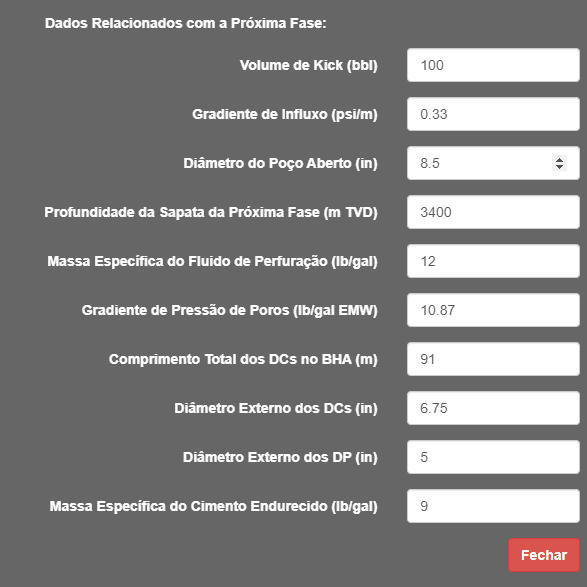
\includegraphics[scale=0.4]{Figures/kickgas.png}
%\vspace{12pt}
\caption{Dados para simulação de um \textit{kick} de gás no CWELL.}
\label{fig:kickgas}
\end{center}
\end{figure}



% --------------------------------------------------------------------------
\section{Resultados e discussão} \label{sec:resultados}
% --------------------------------------------------------------------------

A Tabela \ref{tab_res} apresenta as resistências dos revestimentos de poço obtidas pelo CWELL. Do revestimento condutor ao de produção nota-se uma diminuição da resistência axial. Por outro lado, as resistências por $burst$ e colapso aumentam na direção do revestimento condutor ao de produção. Assim, há uma tendência de os esforços serem mais acentuados por tração no revestimento condutor e de esforços por pressão mais acentuados nos revestimentos intermediário e de produção. 

\begin{table}[H]
\centering
\caption{Resistência das colunas de revestimento.}
\begin{tabular}{c|c|c|c}
Resistência     & \begin{tabular}[c]{@{}c@{}}Revestimento Condutor\\(Tubo H40)\end{tabular} & \begin{tabular}[c]{@{}c@{}}Revestimento Intermediário\\(Tubo K55)\end{tabular} & \begin{tabular}[c]{@{}c@{}}Revestimento de Produção\\(Tubo C75)\end{tabular}  \\ 
\hline
Tração [klbf]   & 1076,71                                                                   & 961,80                                                                         & 698,00                                                                        \\
$Burst$ [psi] & 1533,00                                                                   & 3094,39                                                                        & 8493,75                                                                       \\
Colapso [psi]   & 515,47                                                                    & 1539,51                                                                        & 8201,37                                                                      
\end{tabular}
\label{tab_res}
\end{table}

Na Figura \ref{fig:resultsF1}(a) são apresentadas as envoltórias de resistência e de perda de circulação total no revestimento condutor (Tubo H40). Os esforços pela perda  encontram-se no interior dos limites API e da elipse de von Mises, apontando que as resistências calculadas com base nos fatores de segurança são atendidas, bem como o comportamento constitutivo do tubo em regime elástico, respectivamente. A Figura \ref{fig:resultsF1}(b) demonstra o contrário para o revestimento intermediário (Tubo K55), ou seja, os esforços por perda de circulação em parte da coluna ultrapassam a região segura, indicando riscos à integridade desse revestimento e a necessidade da escolha de um novo tubo.


\begin{figure}[H]
\begin{center}
\center
\subfigure[ref1][]{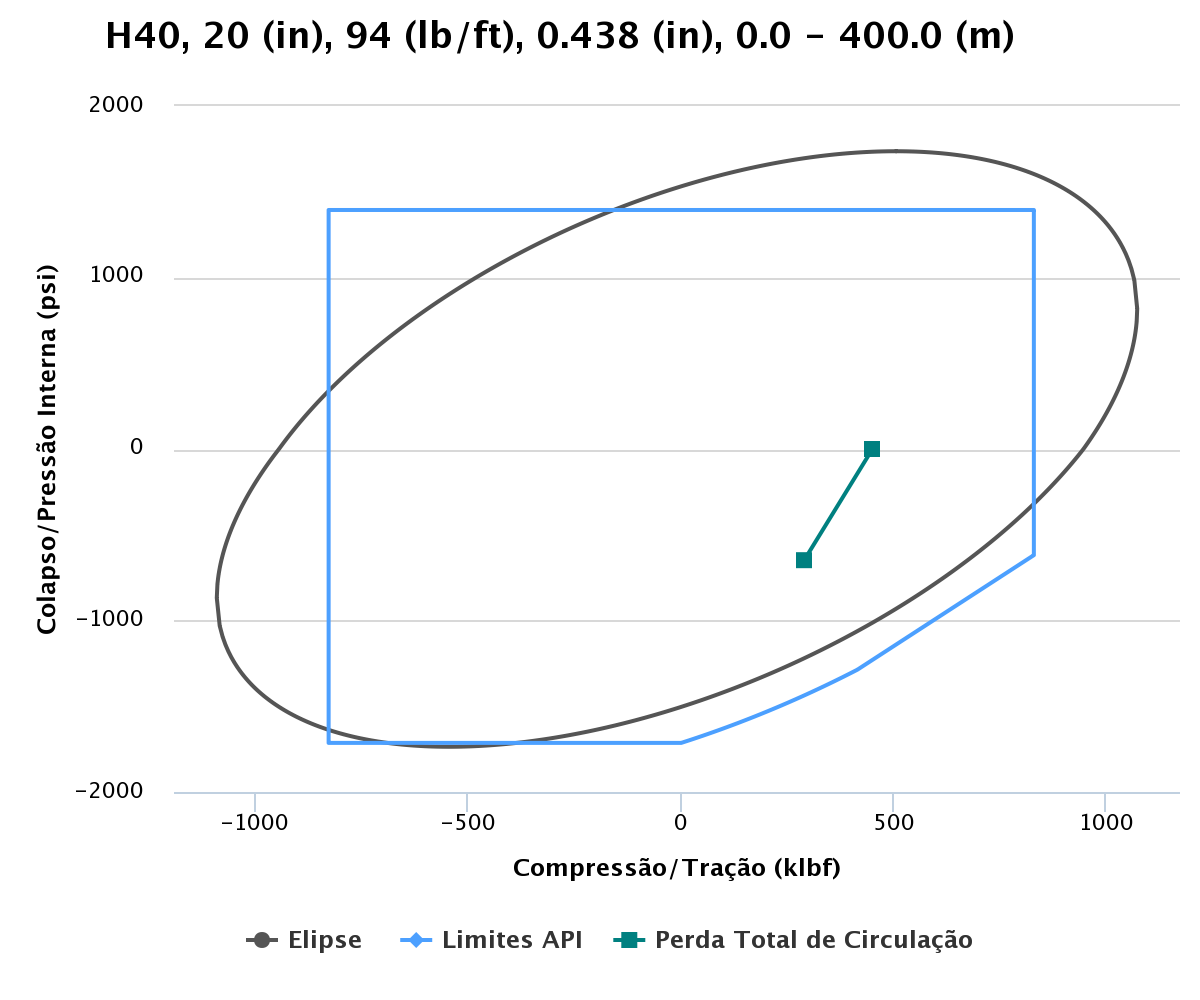
\includegraphics[width=7.6cm]{./Figures/fase1/tri.png}}\qquad
\subfigure[ref2][]{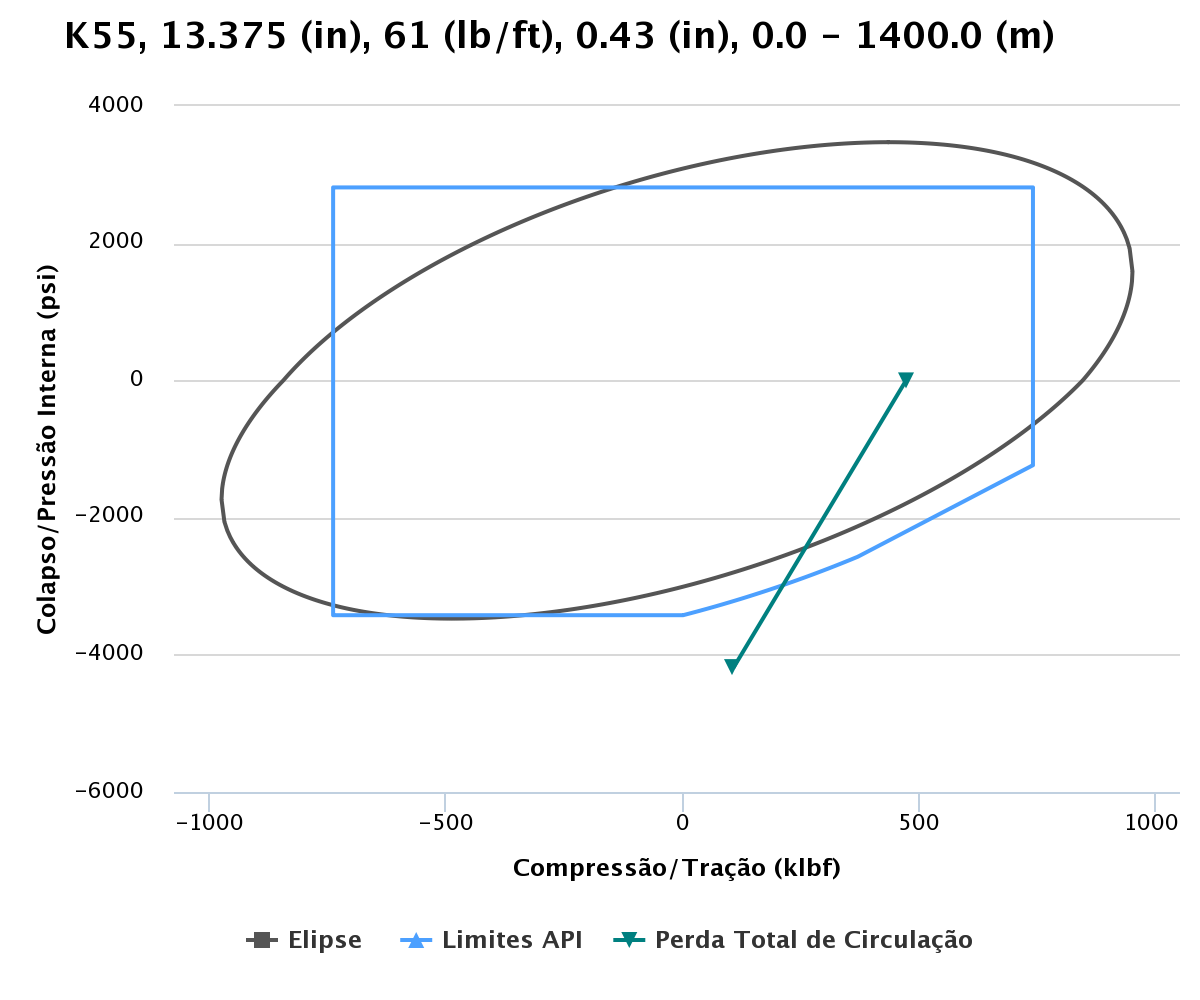
\includegraphics[width=7.6cm]{./Figures/fase2/tri.png}}
%\subfigure[ref3][]{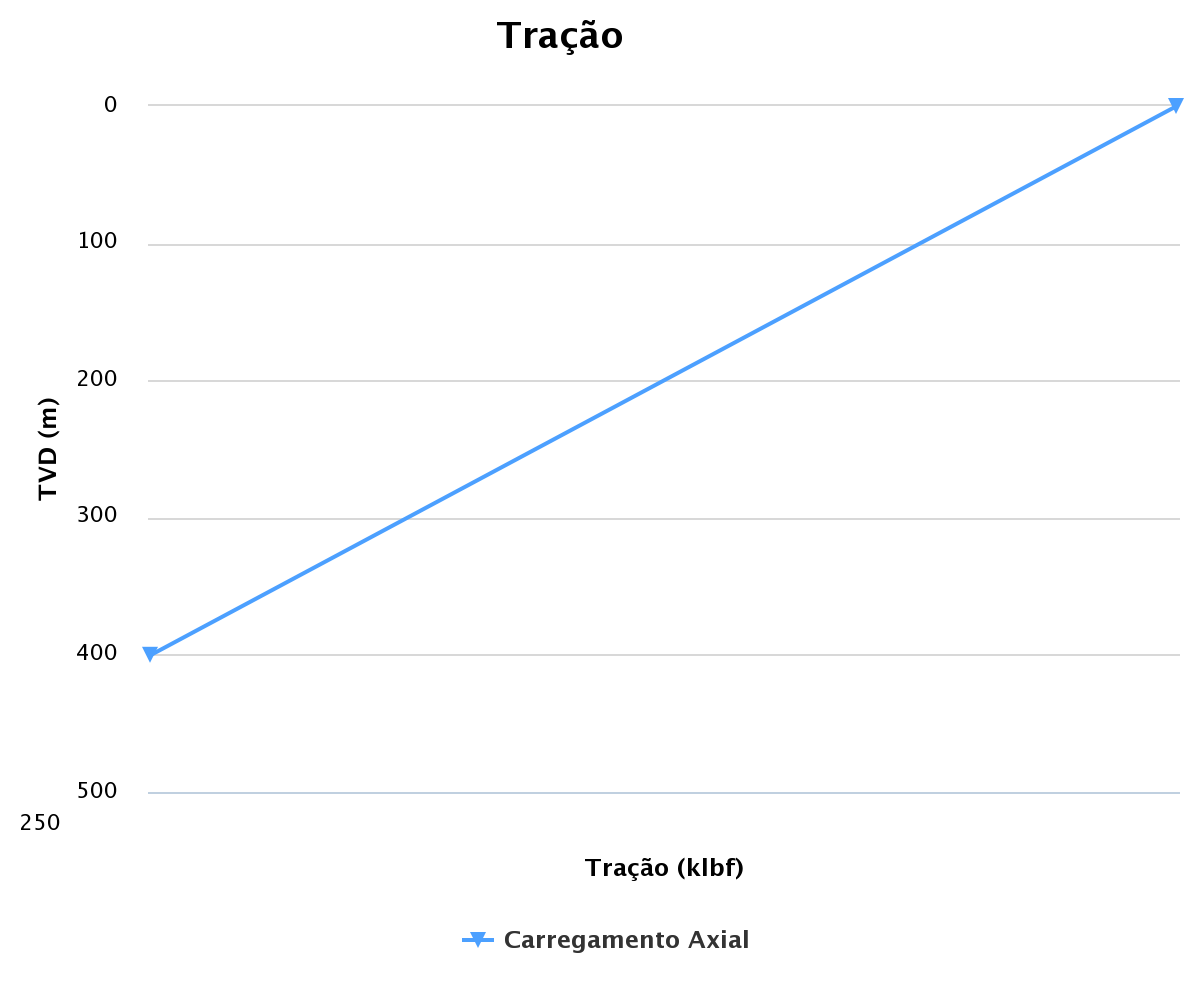
\includegraphics[width=7.6cm]{./Figures/fase1/tracao.png}}
\caption{\centering{Análise triaxial nos revestimentos: (a) condutor e (b) intermediário.}}
\label{fig:resultsF1}
\end{center}
\end{figure}

Neste sentido, são avaliados tubos com grades M65, C75, L80, N80 e C90, de modo que apenas o tubo com a última grade forneceu um resultado exclusivamente no domínio seguro, conforme ilustrado na Figura \ref{fig:resultsF2}(a). Os outros tubos foram evoluindo gradativamente. Aqueles com grades L80 e N80, por exemplo, chegaram a ter o esforço de tração mínimo sobre a elipse de von Mises e os limites do API respeitados, conforme ilustrado na Figura \ref{fig:resultsF2}(b). Porém, sendo bastante rigoroso, haveria a iminência de plastificação. Desta forma, uma sugestão que pode garantir a segurança estrutural e minimizar o custo é a utilização de um revestimento intermediário com seções combinadas. 

\begin{figure}[H]
\begin{center}
\center
\subfigure[ref1][]{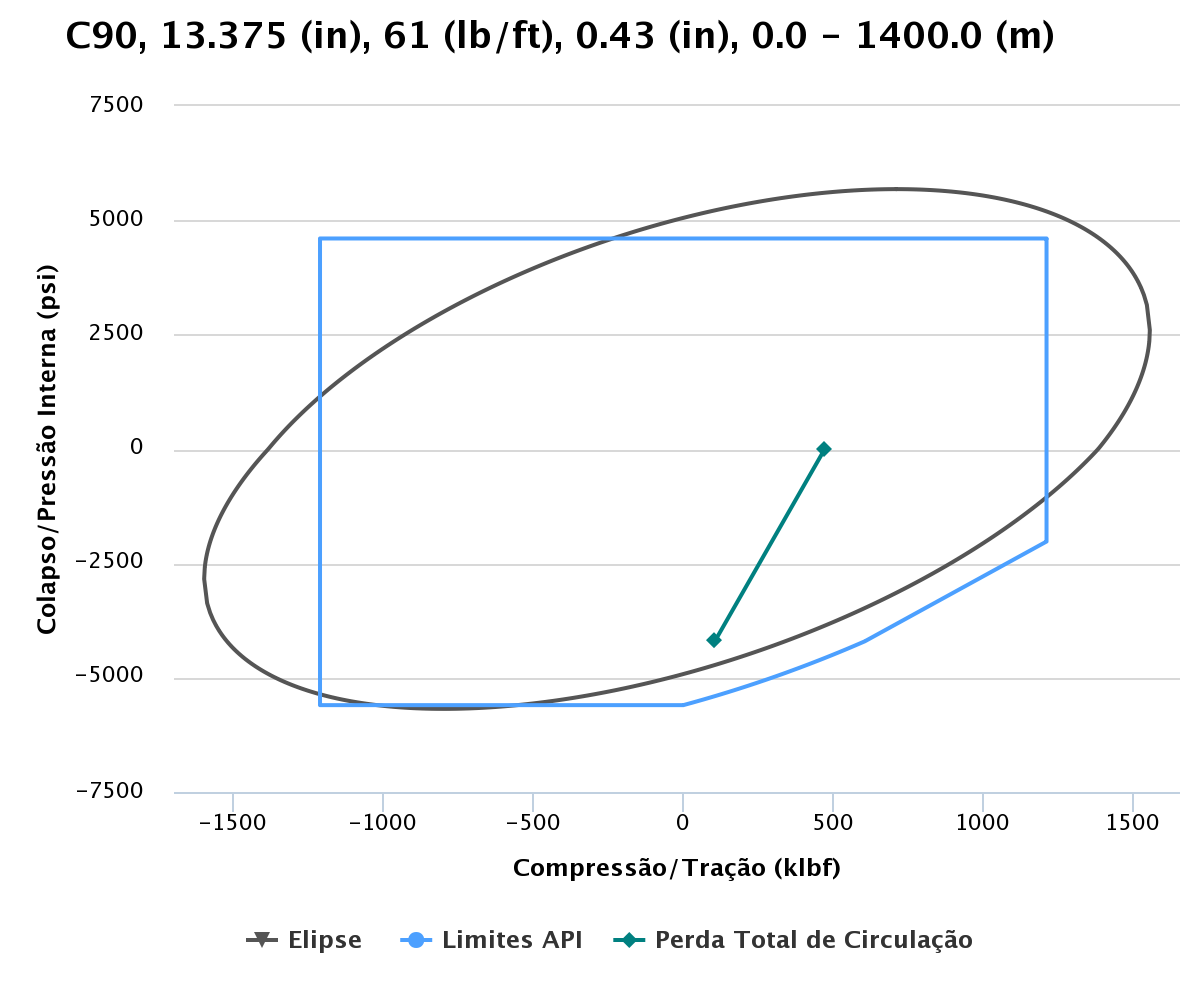
\includegraphics[width=7.6cm]{./Figures/fase2/c90.png}}\qquad
\subfigure[ref2][]{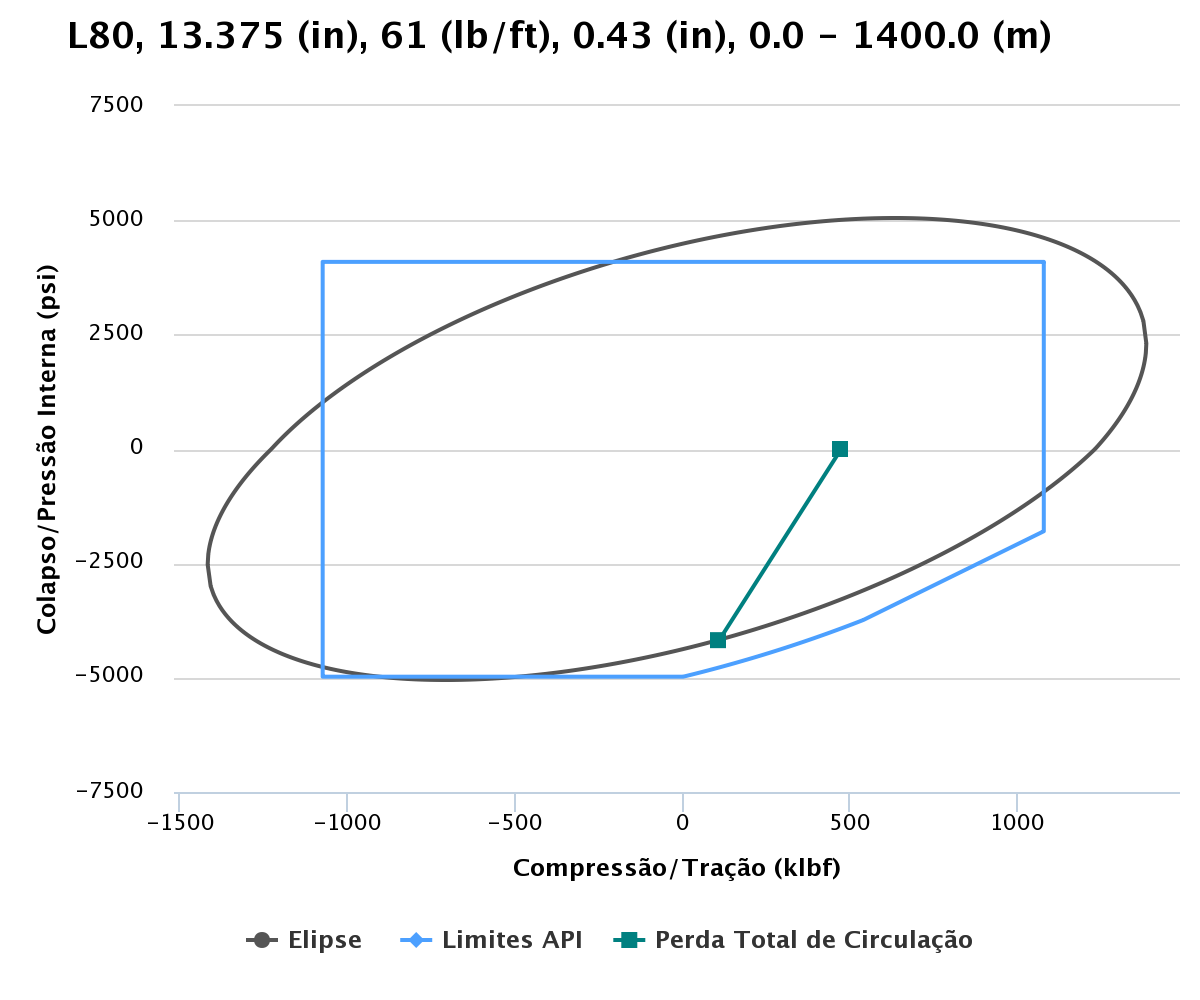
\includegraphics[width=7.6cm]{./Figures/fase2/l80.png}}
%\subfigure[ref3][]{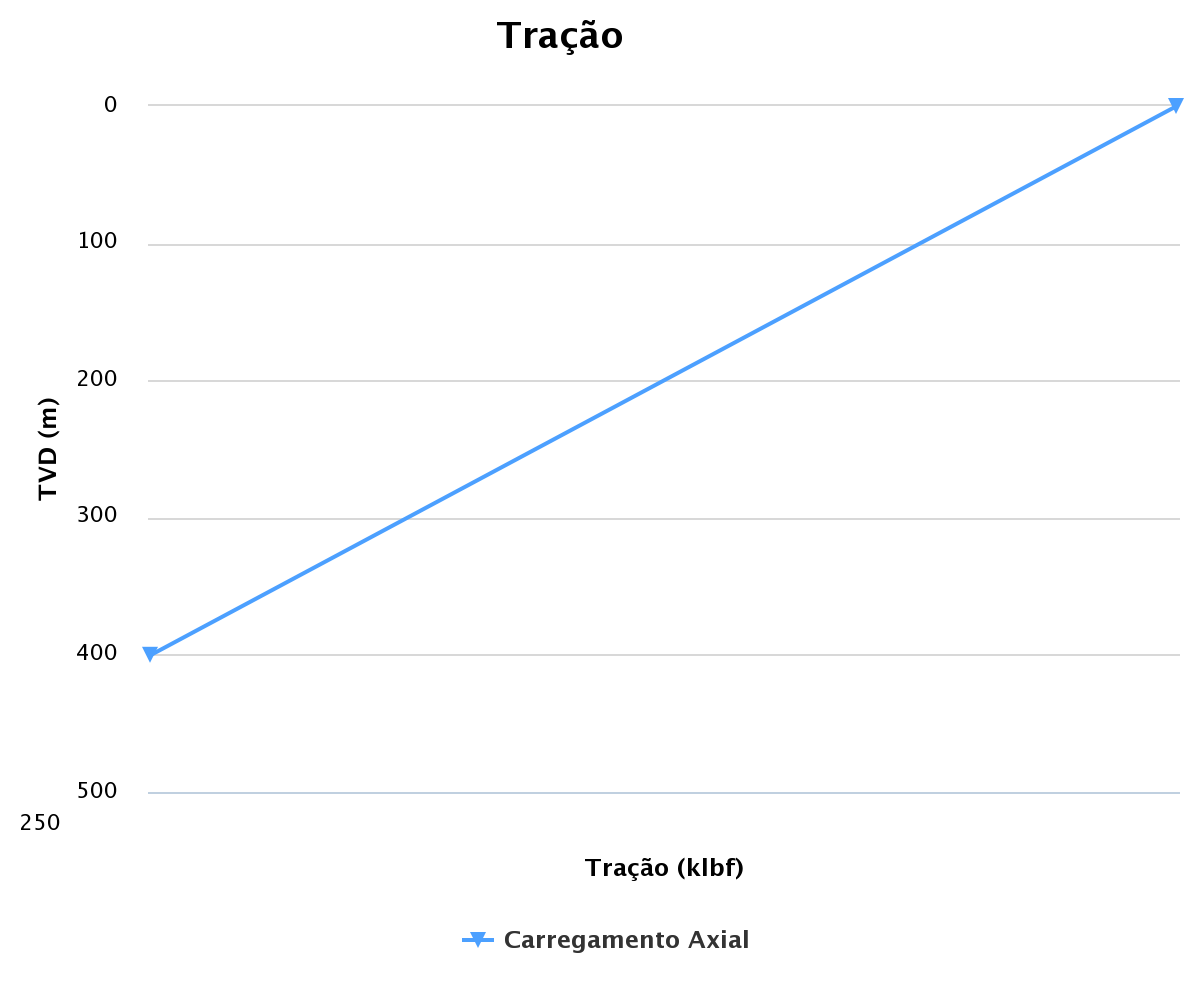
\includegraphics[width=7.6cm]{./Figures/fase1/tracao.png}}
\caption{\centering{Análise triaxial no revestimento intermediário: (a) C90 e (b) L80.}}
\label{fig:resultsF2}
\end{center}
\end{figure}

%\begin{figure}[H]
%\begin{center}
%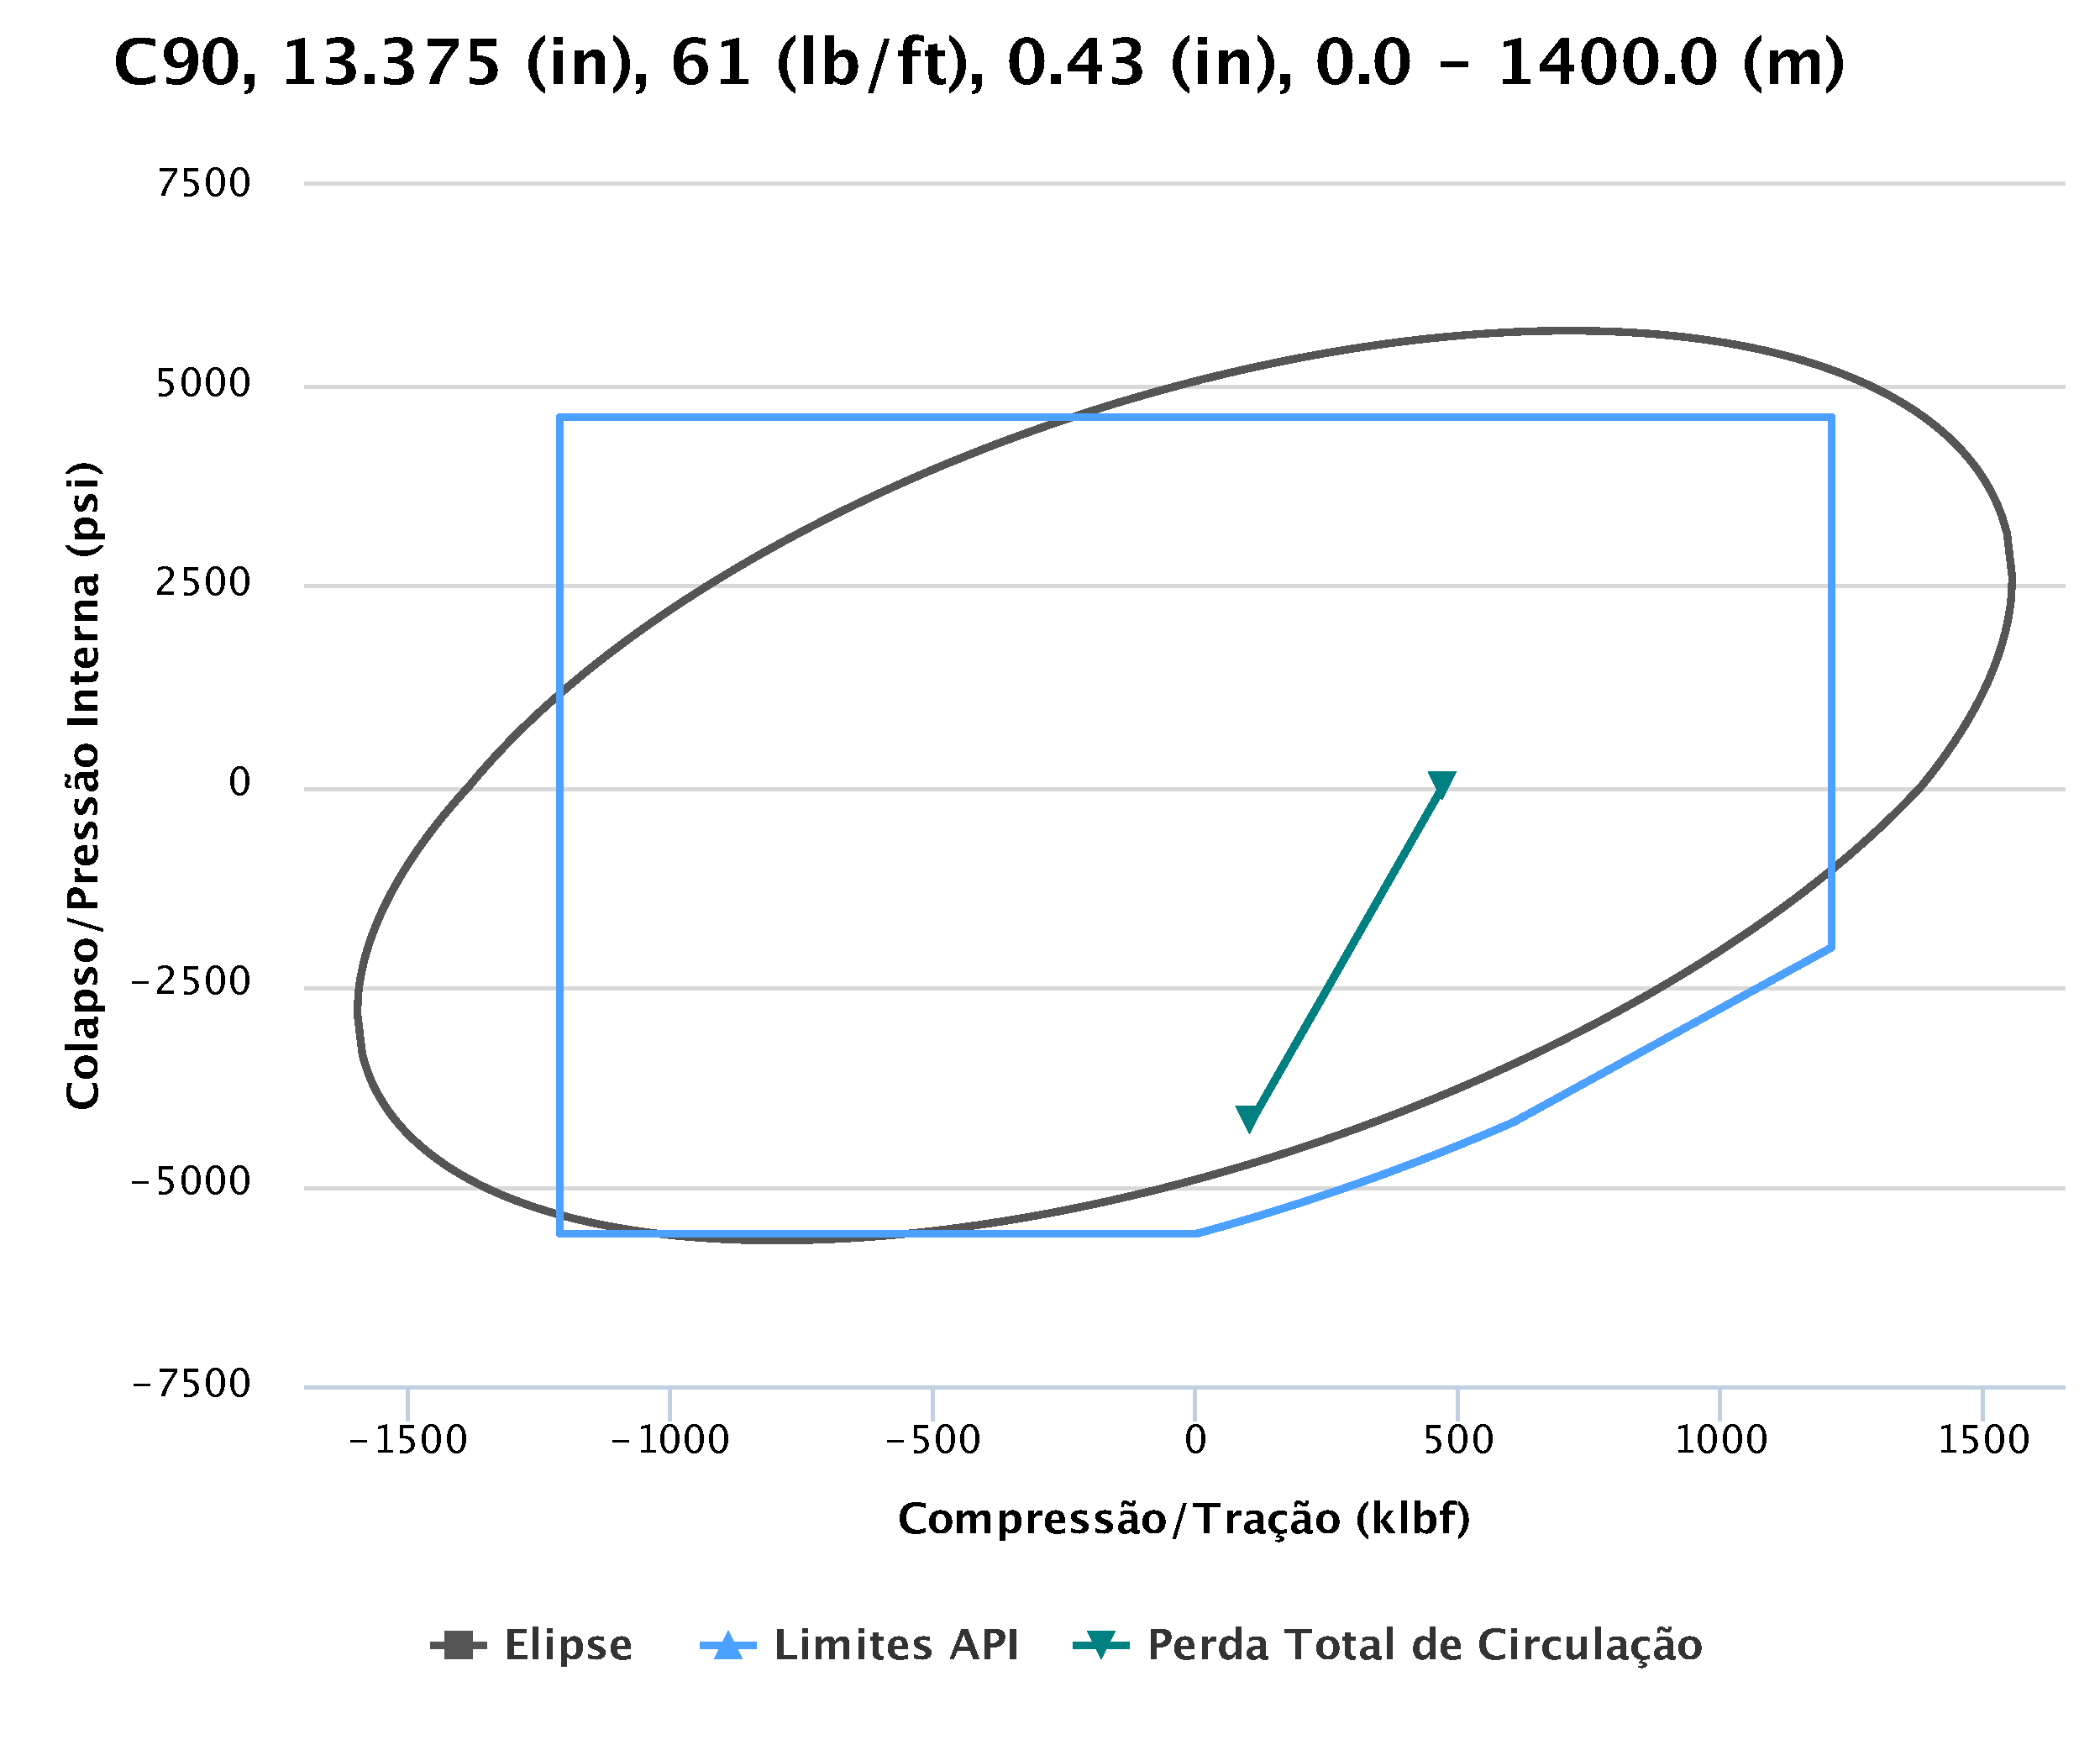
\includegraphics[scale=0.2]{Figures/tubo_proposto_c90.pdf}
%\vspace{12pt}
%\caption{\centering{Proposta de revestimento condutor.}}
%\label{fig:graph}
%\end{center}
%\end{figure}
%\vspace{8pt}

%A Figura \ref{fig:resultsF1}(b) demonstra o contrário para o revestimento intermediário, ou seja, os esforços por perda de circulação em parte da coluna ultrapassam a região segura, indicando riscos à integridade desse revestimento e a necessidade da escolha de um novo tubo. 


\begin{figure}[H]
\begin{center}
\center
\subfigure[ref1][]{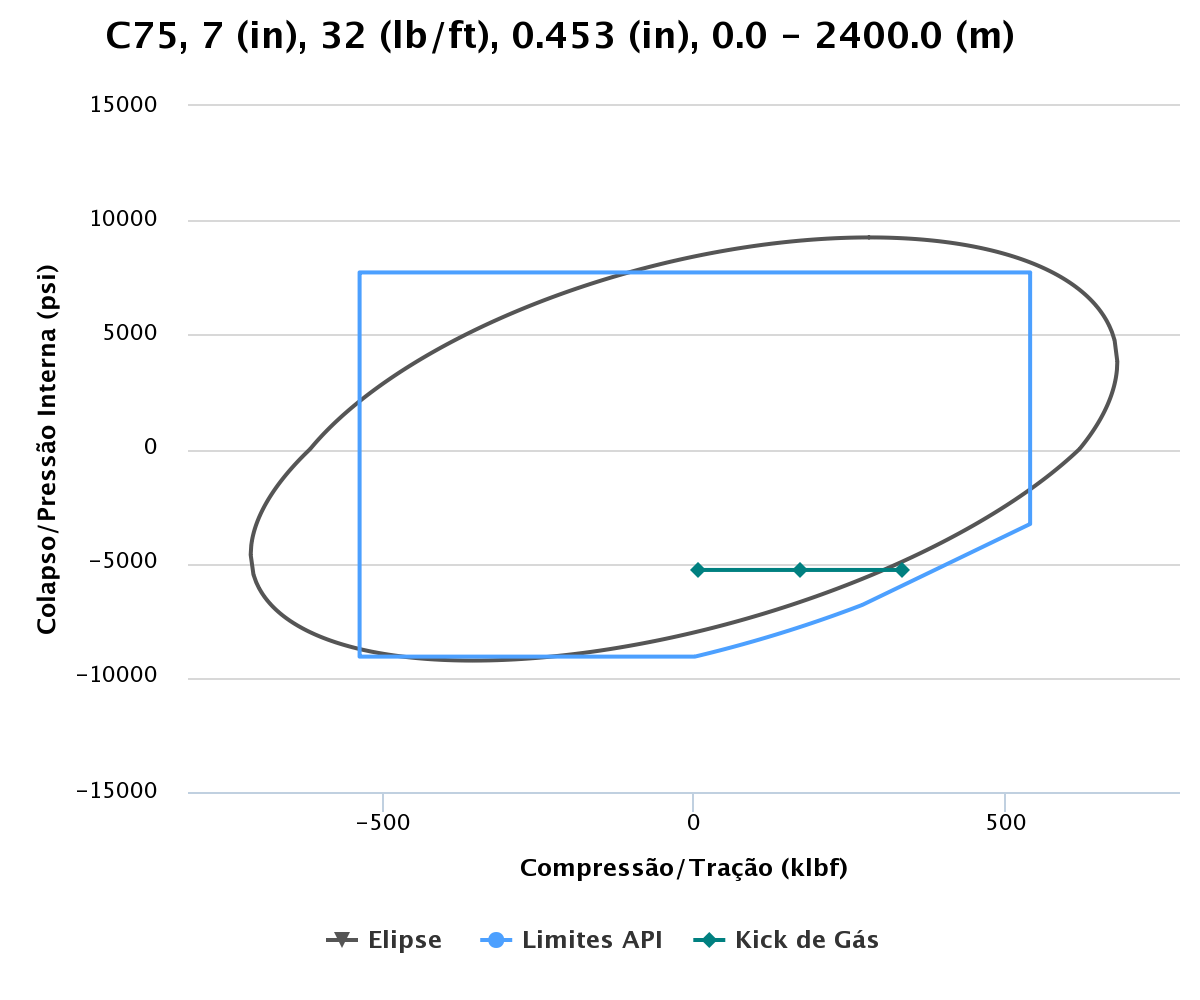
\includegraphics[width=7.6cm]{./Figures/fase3/tri.png}}\qquad
\subfigure[ref2][]{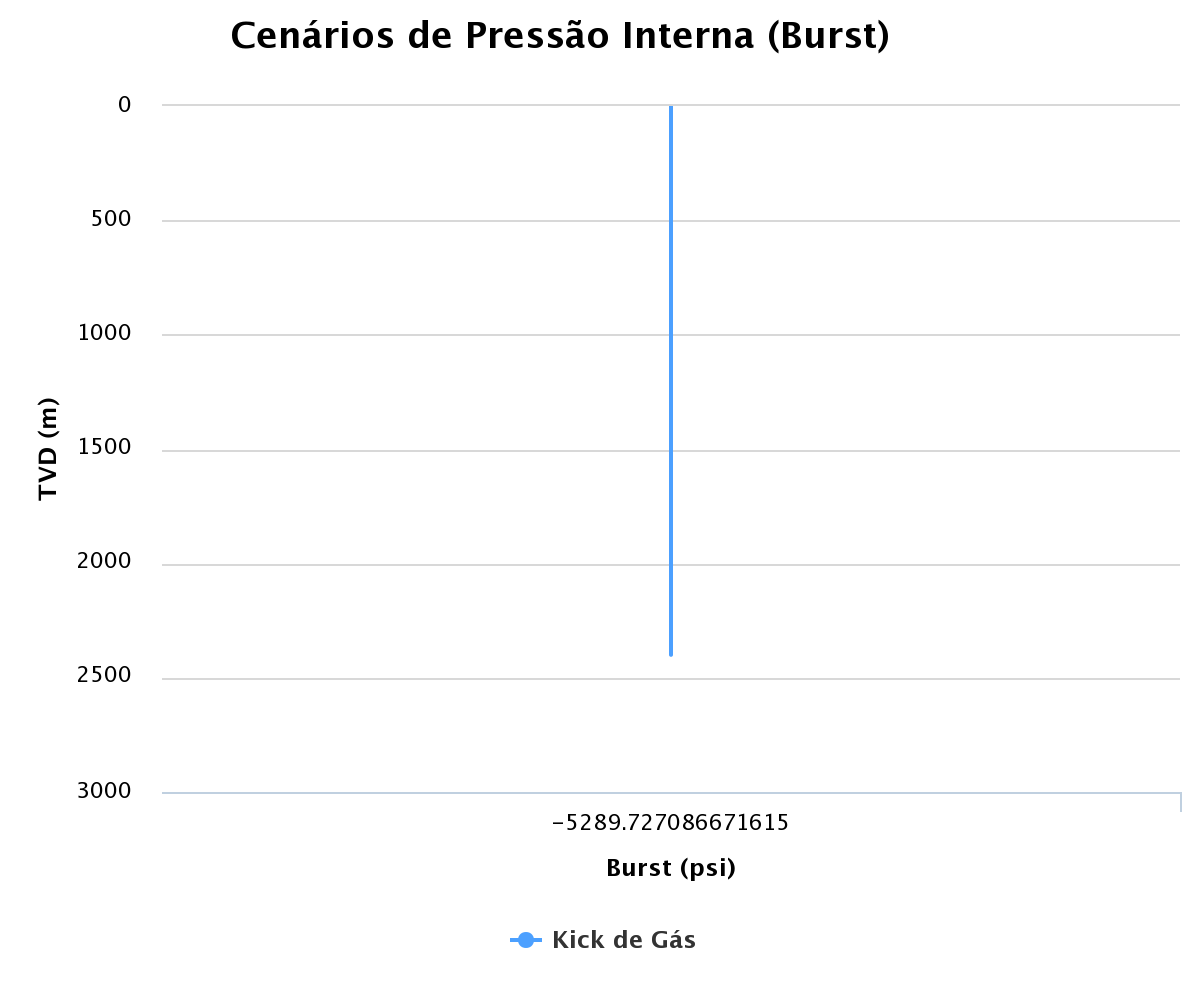
\includegraphics[width=7.6cm]{./Figures/fase3/burst.png}}
\subfigure[ref3][]{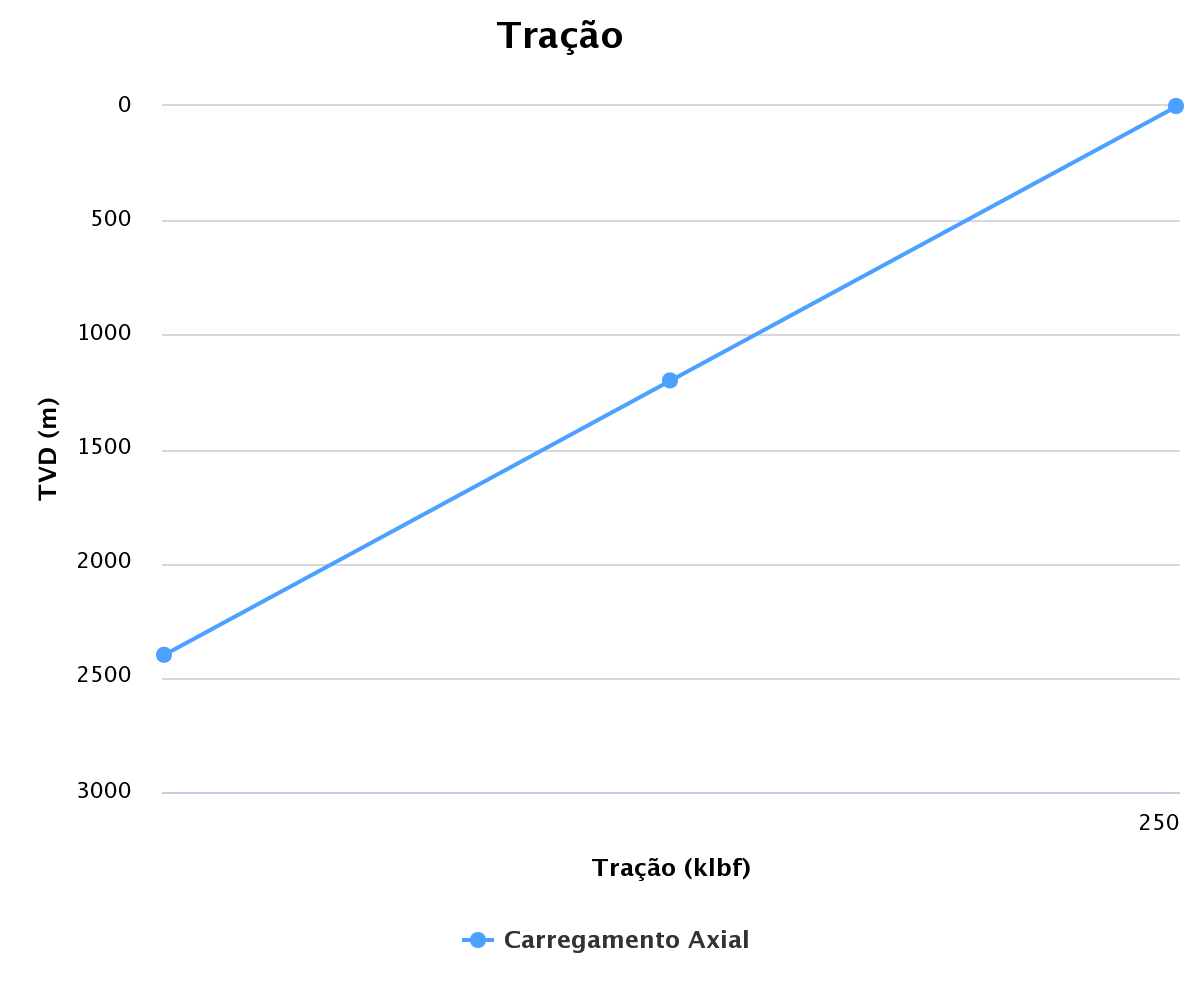
\includegraphics[width=7.6cm]{./Figures/fase3/tracao.png}}
\caption{\centering{Proposta de revestimento condutor.}}
\label{fig:resultsF3}
\end{center}
\end{figure}


% --------------------------------------------------------------------------
\section{Conclusão}\label{sec:Conclusão}
% --------------------------------------------------------------------------







%-------------------------------------------------------------------------
%\vspace{20pt}
%\noindent \textbf{Acknowledgements.} This section should be positioned immediately after the Conclusion section. Type {Acknowledgements} in boldface, 10 pt Times New Roman type from left margin, leaving 20 pt line spacing before and 12pt after.
%\vspace{12pt}

%--------------------------------------------------------------------------
%\noindent \textbf{Authorship statement.} This section is mandatory and should be positioned immediately before the References section. The text should be exactly as follows:  The authors hereby confirm that they are the sole liable persons responsible for the authorship of this work, and that all material that has been herein included as part of the present paper is either the property (and authorship) of the authors, or has the permission of the owners to be included here. 

\bibliography{bibliography}

\end{document}
% --------------------------------------------------------------------------
